
\documentclass[11pt]{article}

\usepackage{common}
\usepackage{hyperref}
\usepackage{amsmath}
\usepackage{listings}
\usepackage{color}

\lstset{frame=tb,
  language=Java,
  aboveskip=3mm,
  belowskip=3mm,
  showstringspaces=false,
  columns=flexible,
  basicstyle={\small\ttfamily},
  numbers=none,
  numberstyle=\tiny\color{gray},
  keywordstyle=\color{blue},
  commentstyle=\color{dkgreen},
  stringstyle=\color{mauve},
  breaklines=true,
  breakatwhitespace=true,
  tabsize=2
}

\definecolor{dkgreen}{rgb}{0,0.6,0}
\definecolor{gray}{rgb}{0.5,0.5,0.5}
\definecolor{mauve}{rgb}{0.58,0,0.82}
% credit to http://stackoverflow.com/questions/3175105/writing-code-in-latex-document

\title{CS262 Final Project: Remote Procedure Calls for Data Science}
\author{Andrew Mauboussin \\ ammaub@college.harvard.edu}
\begin{document}

\maketitle{}

Code and documentation at \textcolor{blue}{ \href{https://github.com/amauboussin/ds-rpc}{https://github.com/amauboussin/ds-rpc}}\\\\
\indent I affirm my awareness of the standards of the Harvard College Honor Code.



\section{Abstract}
This paper presents a system for calling scientific computing functions remotely. The system is structured similar to previous RMI/RPC systems with a small number of types (numerical primitives and multi-dimensional arrays). The small interface allows multi-language serialization/de-serialization using JSON (client libraries are provided for Python and JavaScript and could quickly be implemented in other languages). Code is not sent over the network; instead, the server exposes scientific computing functions from various Python/R libraries (numpy, scipy, gtools, etc.). The system could prove useful for running scientific computing functions on devices where it is impractical to install the appropriate libraries or reimplement the required functionality  without having to implement a custom interface and think about message passing/serialization. 

\section{Introduction}

There are several reasons why it may be necessary to run code remotely for data intensive applications. First, it may not be practical to store all the necessary data in the memory of one machine. This problem has motivated a variety of ``big data" systems that perform computations over partitioned data, including Google MapReduce and Apache Spark. Second, it may not be practical to run execute code on a given machine, either because it would be too slow or because it would be cumbersome to install or reimplement functionality from a given library. 

Today, this problem is often solved through the implementation of a custom API. The wide availability of standard implementations for serialization (JSON, Protocol Buffers) and web frameworks (Rails, Django, Node) that allow easy message passing over the Internet continue to make this solution an attractive option. But implementing a custom API inevitably means defining, documenting, and maintaining an interface, which can be a lot of work. Another option is abstracting out the serialization and message passing with a system like RMI. After a bit of configuration, these systems allows programmers to call remote functions the same way they call local ones (just add an extra line or two to catch the remote exception). However, the abstractions they provide make multi-language support using these systems difficult - they are typically forced to take the set intersection of types between the supported languages or maintain a custom interface between types. 

``Data science RPC" is a new system that provides a multi-language abstraction over serialization and message sending by maintaining a narrow scope. The system allows users to remotely run methods from a variety of scientific computing libraries in Pyhon and R. The inspiration for the project comes from the observation that most scientific computing libraries are primarily around matrix/multi-dimensional array types and numerical primitives. By limiting the scope of the project to scientific computing functions, many of the challenges that are typically with multi-langauge message passing and serialization abstractions are avoided. In other words, the system is able to ignore the hardest problems in remote procedure call systems (serializing code/custom classes, inter-language conversion) by limiting its scope and only attempting to provide an interface for remote scientific computing rather than arbitrary code execution. 

\section{System Overview}


\begin{figure}[!ht]
  \centering
      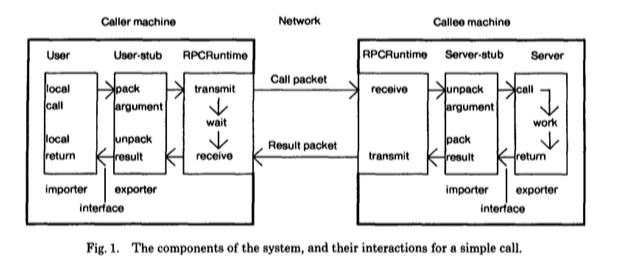
\includegraphics[width=0.8\textwidth]{stubs}
  \caption{Overview of the stub system (Figure 1 in the Birrell and Nelson paper)}
\end{figure}

The system's structure is inspired by Birrell and Nelson's ``stub system" (shown above). There are three main components involved in each call: the client (or user) stub, the network, and the server stub. When a client wants to run a remote computation, they can use a simple interface provided by the client stub. The interface includes the language of the desire computation, the function to be run (selected from one of the libraries installed on the server), and any arguments that the function takes (server.python(function\_name, function\_arg1, function\_arg 2...), see documentation for more details).  The client stub will then turn this function call into an HTTP request that includes the version number of the protocol, the language and function of the requested computation, and JSON versions of each of the arguments. The request is sent over the network to the server, which parses it, runs the relevant computation, serializes the result in JSON, and then sends it back to the client. Finally, the client stub deserializes the result and returns in to the user. 

The current implementation of the project includes client stubs for Python and JavaScript and server stubs for Python and R. In this implementation, the server stub are running on a Flask app in Python and each take the same arguments. The R stub is implemented by ``shelling out" from Python (invoking a command line script from within Python). Server stubs for other languages could work in a similar way. 

The client stubs are relatively thin wrappers that present a language-specific interface to the user and then serialize request so it can be sent to the server. Ideally, each client library will follow the paradigms of the language it is written in to ``blend in" with other libraries in that language and allow a consistent experience to users.  For example, the Python client library sends requests synchronously (waits until it receives a response) whereas the JavaScript client library sends requests asynchronously (doesn't wait after sending a request) and then sends the results to a callback. However, both client libraries ultimately send the same requests to the server. Including client libraries allows the system to feel native in each of the languages it is available in. Example usage in both the Python and JavaScript is shown below. 

\begin{figure}[!ht]
  \centering
     \lstset{language=Python}
\begin{lstlisting}
from ds_rpc import Server
server = Server() # url set settings.json
# sample from a Dirichlet distribution with uniform alpha
ones = [1 for _ in range(3)]
n_samples = 3
result = server.r('gtools.rdirichlet', n_samples, ones)
print result
# returns [[[0.0606,0.1637,0.095,0.6807],
# [0.0625,0.6069,0.2534,0.0773],
# [0.2252,0.2347,0.0306,0.5095]]]
\end{lstlisting}  \caption{Sampling from a Dirichlet distribution in R using the Python client library. }
\end{figure}


\begin{figure}[!ht]
  \centering
\lstset{language=Java}
\begin{lstlisting}
// calculate the correlation coefficient between two lists of random numbers
var server = new Server(server_url);
var callback = function(result){console.log(result);}
var x = get_n_random_numbers(100); //gets a list of 100 random numbers between 0 and 1
var y = get_n_random_numbers(100);
server.python(callback, 'scipy.stats.pearsonr', x, y);

// outputs [0.09398385492166901,0.3523279903811445]
// (the scipy pearsonr function returns the correlation constant and the p value)
\end{lstlisting}  \caption{Calculating a correlation coefficent in Python using the JavaScript client library. }
\end{figure}


A longer demo is available in the linked Github repository. Examples using the JavaScript client library can be found by launching the server and then navigating to /demo in a browser (or just opening static\_demo.html to see sample output without any setup). Examples using the Python client library are in python-client/test\_client.py (running it will print function being called and the output).

\section{Limitations}

Data science RPC is a relatively simple system that leverages JSON, HTTP, and scientific computing libraries in order to allow remote code execution with a relatively simple design. Each of these design choices comes with limitations. The most important decisions and their implications are discussed below.

\subsection{Short list of types}

The short list of types is what makes cross-language support possible. Right now, the system only supports ints, floats, strings, and multi-dimensional arrays of an type. Because the list of supported types is small, it is possible to maintain a serializer/deserializer between the RPC types and each of language-specific types. Unfortunately, restricting the type system also limits what functions can be used. For example, most integration and optimization routines take the function being integrated/optimized as an argument. Since the system has no way to serialize functions, these cannot be used. 

Even with the current short list of types, there could possibly source of trouble is the server deserialization when the stub decides what type to load each multi-dimensional array in. For example, in Python, it could conceivably use either Numpy arrays or lists whereas in R it could use an Array or a more specific type like a time series or a matrix. Right now, the system uses sensible defaults that cover most cases. In the future, the client libraries could be modified to take optional arguments ``arg1\_type", ``arg2\_type", etc. to denote how each argument should be deserialized if the default option isn't correct. This would enable things like casting a multi-dimensional array to an R time series so time series functionality could be used. 

\subsection{JSON serialization}

Another important design decision was the use of JSON serialization rather than a binary format. This made development easier because I could use existing libraries for JSON serialization rather than having to write my own custom serialization/deserialization code for each type in the system. It also means that the messages are easily sent over HTTP (Flask, the web framework I used to write the server, has explicit support for sending JSON) and are human-interpretable. However, JSON does come with a relatively large performance tradeoff. Marshaling/unmarshaling binary formats is potentially much faster and uses much less space than a text-based solution like JSON. The difference can add up quickly because each call to the RPC server requires four serializations/deserializations (serialize arguments, deserialize arguments, serialize results, deserialize results) in addition to a round trip over the network. Choosing a binary format could like result in around an order of magnitude of improvement and make the system usable with substantially larger amounts of data. 


\subsection{No running custom code}

Instead of requiring users to register code, the system exposes the global namespace and any installed libraries of Python and R.This has a few advantages. First, it makes set up easy. Any functionality on the server is available out-of-the-box and each ds-rpc server is identical (assuming the same libraries are installed on each box). Second, all of the documentation for the available functions is easily accessible online. The one thing that is not currently easy to find is the list of available libraries/functions (one useful add-on would be a function that returns all available libraries to clients). The clear disadvantage to sticking with libraries is a lack of flexibility - if more complicated tasks need to be executed, it is likely easier to just build a custom interface. This problem could be alleviated by adding more options to the current interface. For example, it would be useful if users could compose functions from libraries without requiring a round-trip over the network. It would also be nice to have pre-built interfaces for common tasks, like training and running cross-validation on a classifier model.

\section{Conclusion}

Data Science RPC provides a simple interface for remotely executing code form scientific computing libraries, but is constrained by the some of the design choices. Because JSON serialization is not very performant and transferring large amounts of data over the network would be slow, the system is most likely to be useful if either the computation being run is very expensive or if the computer that needs the result is very slow. One possible application is in the ``Internet of things". It may be useful to be able leverage Python/R scientific computing libraries on devices like a ``smart" refrigerator or thermostat with low-level environments. It may also be useful for running expensive computations on mobile devices.

Despite its potential usefulness the system is not quite ready for the prime time yet. As mentioned above, the short list of types and lack of custom code restricts the scope of the computations that can be run. The JSON serialization also limits performance. However, expanding the scope of the project would likely prove to be very difficult/a lot of work: handling automatic serialization for a small range of types is achievable, but as the number of types increases it results in a combinatorial explosion in the number of cases (as serializers from/to every type in each supported language and RPC type need to be supported). It would also be difficult to keep on top of each case as the underlying languages evolved. In other words, maintaining a large interface is fundamentally difficult so we may be stuck with hand-crafted APIs or small but generalizable APIs (like this project) for the conceivable future. 


\bibliographystyle{apalike}
\bibliography{writeup}

\end{document}
